\documentclass[12pt, a4paper]{book}

\usepackage[T1]{fontenc}
\usepackage[utf8]{inputenc}
\usepackage[charter, cal=cmcal]{mathdesign}
\usepackage[scaled=0.92]{helvet}
\usepackage{geometry}
\geometry{a4paper, top=30mm, bottom=30mm, inner=32mm, outer=25mm, marginparwidth=18mm}

\usepackage{amsmath, amsthm}
\usepackage[version=4]{mhchem}
\usepackage{graphicx}
\usepackage[dvipsnames,svgnames,table]{xcolor}
\usepackage{tikz}
\usetikzlibrary{arrows.meta, shapes.geometric, positioning, calc, backgrounds}
\usepackage{pgfplots}
\pgfplotsset{compat=1.18}
\usepackage{tcolorbox}
\tcbuselibrary{skins, breakable, theorems}
\usepackage{titlesec}
\usepackage{fancyhdr}
\usepackage{enumitem}
\usepackage{booktabs}
\usepackage{array}
\usepackage{multicol}
\usepackage{caption}
\usepackage{parskip}
\usepackage{siunitx}
\usepackage{pifont}
\usepackage{colortbl}
\usepackage[colorlinks=true, linkcolor=BrickRed,
            urlcolor=NavyBlue, citecolor=ForestGreen]{hyperref}

% ── Colours (Journey 3) ───────────────────────────────────────────────────────
\definecolor{JourneyColor}{HTML}{145A32}
\definecolor{ModuleColor}{HTML}{1E8449}
\definecolor{PuzzleColor}{HTML}{1A5276}
\definecolor{DiscoveryColor}{HTML}{B7950B}
\definecolor{WarningColor}{HTML}{C0392B}
\definecolor{ProblemColor}{HTML}{4A235A}
\definecolor{ReflectColor}{HTML}{117A65}
\definecolor{HistoryColor}{HTML}{6E2F1A}
\definecolor{TrendDown}{HTML}{1A5276}
\definecolor{TrendUp}{HTML}{922B21}
\definecolor{ShieldGray}{HTML}{566573}

% ── Boxes ─────────────────────────────────────────────────────────────────────
\newtcolorbox{puzzlebox}[1][]{enhanced,breakable,
  colback=PuzzleColor!6,colframe=PuzzleColor,fonttitle=\bfseries\sffamily,
  title={The Puzzle},attach boxed title to top left={yshift=-2mm,xshift=6mm},
  boxed title style={colback=PuzzleColor},borderline west={3pt}{0pt}{PuzzleColor},#1}

\newtcolorbox{discoverybox}[1][]{enhanced,breakable,
  colback=DiscoveryColor!8,colframe=DiscoveryColor,fonttitle=\bfseries\sffamily,
  title={Discovery},attach boxed title to top left={yshift=-2mm,xshift=6mm},
  boxed title style={colback=DiscoveryColor},borderline west={3pt}{0pt}{DiscoveryColor},#1}

\newtcolorbox{problembox}[1][]{enhanced,breakable,
  colback=ProblemColor!5,colframe=ProblemColor,fonttitle=\bfseries\sffamily,
  title={Problems},attach boxed title to top left={yshift=-2mm,xshift=6mm},
  boxed title style={colback=ProblemColor},borderline west={3pt}{0pt}{ProblemColor},#1}

\newtcolorbox{deepbox}[1][]{enhanced,breakable,
  colback=JourneyColor!5,colframe=JourneyColor,fonttitle=\bfseries\sffamily,
  title={Deep Problems},attach boxed title to top left={yshift=-2mm,xshift=6mm},
  boxed title style={colback=JourneyColor},borderline west={4pt}{0pt}{JourneyColor},#1}

\newtcolorbox{historybox}[1][]{enhanced,breakable,
  colback=HistoryColor!7,colframe=HistoryColor!60,fonttitle=\bfseries\sffamily\small,
  title={Historical Note},attach boxed title to top left={yshift=-2mm,xshift=6mm},
  boxed title style={colback=HistoryColor!80},#1}

\newtcolorbox{reflectionbox}[1][]{enhanced,breakable,
  colback=ReflectColor!6,colframe=ReflectColor,fonttitle=\bfseries\sffamily,
  title={Reflection},attach boxed title to top left={yshift=-2mm,xshift=6mm},
  boxed title style={colback=ReflectColor},borderline west={3pt}{0pt}{ReflectColor},#1}

\newtcolorbox{namedconcept}[2][]{enhanced,
  colback=ModuleColor!6,colframe=ModuleColor,fonttitle=\bfseries\sffamily\large,
  title={#2},attach boxed title to top left={yshift=-2mm,xshift=6mm},
  boxed title style={colback=ModuleColor},#1}

% ── Section formatting ────────────────────────────────────────────────────────
\titleformat{\chapter}[display]
  {\normalfont\sffamily\huge\bfseries\color{JourneyColor}}
  {\textcolor{JourneyColor!60}{\chaptertitlename\ \thechapter}}{10pt}{\Huge}
  [\vspace{2pt}\textcolor{JourneyColor}{\titlerule[1.5pt]}]
\titleformat{\section}
  {\normalfont\sffamily\Large\bfseries\color{ModuleColor}}
  {\thesection}{1em}{}[\textcolor{ModuleColor!40}{\titlerule[0.6pt]}]
\titleformat{\subsection}
  {\normalfont\sffamily\large\bfseries\color{JourneyColor!80}}{\thesubsection}{1em}{}
\titleformat{\subsubsection}
  {\normalfont\sffamily\normalsize\bfseries}{\thesubsubsection}{1em}{}

\pagestyle{fancy}
\fancyhf{}
\fancyhead[LE]{\small\sffamily\textcolor{JourneyColor}{\leftmark}}
\fancyhead[RO]{\small\sffamily\textcolor{ModuleColor}{\rightmark}}
\fancyfoot[C]{\small\thepage}
\renewcommand{\headrulewidth}{0.4pt}

\newcommand{\newterm}[1]{\textit{\textcolor{DiscoveryColor}{#1}}}
\newcommand{\important}[1]{\textcolor{ModuleColor}{\textbf{#1}}}

% ══════════════════════════════════════════════════════════════════════════════
\begin{document}
\setcounter{chapter}{2}
\chapter[Journey 3 --- The Periodic Table as a Discovery Engine]
        {Journey Three\\[8pt]
         \textcolor{ModuleColor}{\large The Periodic Table as a Discovery Engine}}
\setcounter{section}{1}

% ══════════════════════════════════════════════════════════════════════════════
\section{Module 3.2 --- Periodic Trends: Reading the Table Quantitatively}
\label{sec:mod3.2}

\subsection*{Motivation}

The periodic table is not just a list of elements ---
it is a quantitative map.
Every position encodes a cluster of measurable properties
that change in predictable directions as you move
across a period or down a group.

Once you understand these trends, the table becomes
a calculator: given an element's position,
you can estimate its ionisation energy,
its atomic radius, the bond it will form,
and the compounds it will make ---
\emph{before looking up a single number}.

This module builds that calculator,
explaining each trend from its quantum mechanical origin.

% ─── Section: Effective Nuclear Charge ───────────────────────────────────────
\subsection{The Central Concept: Effective Nuclear Charge}

All periodic trends reduce to one idea:
the \newterm{effective nuclear charge} $Z_\text{eff}$.

An electron in a multi-electron atom does not feel
the full charge of the nucleus.
Inner electrons partially \newterm{shield} (or screen)
the outer electrons from the nuclear charge.

\begin{namedconcept}{Effective Nuclear Charge}
\[
  Z_\text{eff} = Z - S
\]
where $Z$ is the true nuclear charge (atomic number)
and $S$ is the \newterm{shielding constant} ---
the effective number of nuclear charges cancelled
by inner electrons.

An outer electron behaves approximately as if it were
in a hydrogen-like atom with nuclear charge $Z_\text{eff}$.
\end{namedconcept}

\vspace{0.5em}

The key rules for shielding (Slater's rules, simplified):
\begin{itemize}[nosep, leftmargin=2em]
  \item Electrons in lower shells ($n' < n$) shield nearly
        perfectly: each contributes $\approx 0.85$--$1.0$ to $S$.
  \item Electrons in the \emph{same} shell shield poorly:
        each contributes $\approx 0.35$ to $S$.
  \item $s$ orbitals penetrate to the nucleus better than
        $p$, which penetrate better than $d$ or $f$:
        this causes the $s < p < d < f$ energy ordering
        within a shell.
\end{itemize}

\begin{center}
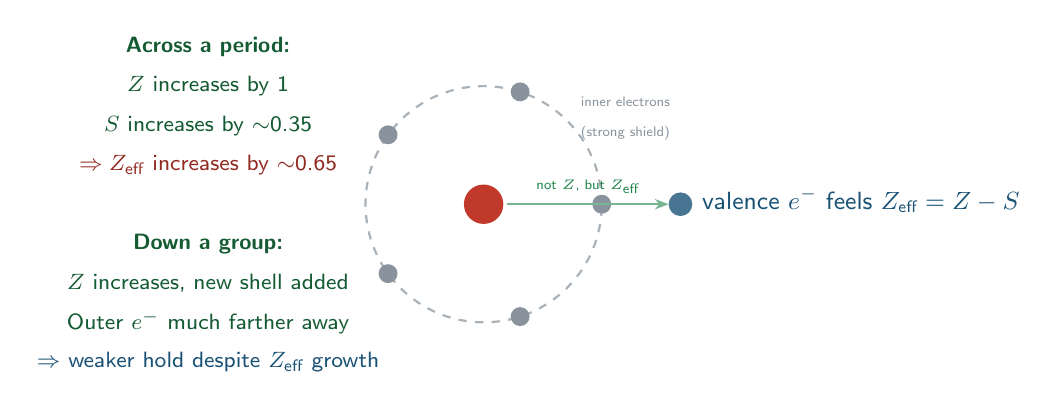
\begin{tikzpicture}[every node/.style={font=\sffamily\small}, scale=1.0]

  % Nucleus
  \fill[WarningColor] (0,0) circle (0.25cm);
  \node[font=\sffamily\small\bfseries, text=WarningColor] at (0,0) {$Z$};

  % Inner shell (n=1,2) - full shield
  \draw[thick, ShieldGray!50, dashed] (0,0) circle (1.5cm);
  \foreach \angle in {0, 72, 144, 216, 288} {
    \fill[ShieldGray!70] ({1.5*cos(\angle)},{1.5*sin(\angle)}) circle (0.12cm);
  }
  \node[font=\sffamily\tiny, text=ShieldGray!70] at (1.8, 1.3)
    {inner electrons};
  \node[font=\sffamily\tiny, text=ShieldGray!70] at (1.8, 0.9)
    {(strong shield)};

  % Outer electron
  \fill[TrendDown!80] (2.5, 0) circle (0.15cm);
  \node[font=\sffamily\small, text=TrendDown, right] at (2.65, 0.05)
    {valence $e^-$ feels $Z_\text{eff} = Z - S$};

  % Arrow showing reduced charge
  \draw[-{Stealth[length=5pt]}, thick, ModuleColor!60]
    (0.3,0) -- (2.35,0)
    node[midway, above, font=\sffamily\tiny, text=ModuleColor]
      {not $Z$, but $Z_\text{eff}$};

  % Two cases
  \node[font=\sffamily\footnotesize\bfseries, text=JourneyColor]
    at (-3.5, 2.0) {Across a period:};
  \node[font=\sffamily\footnotesize, text=JourneyColor]
    at (-3.5, 1.5) {$Z$ increases by 1};
  \node[font=\sffamily\footnotesize, text=JourneyColor]
    at (-3.5, 1.0) {$S$ increases by $\sim$0.35};
  \node[font=\sffamily\footnotesize, text=TrendUp]
    at (-3.5, 0.5) {$\Rightarrow Z_\text{eff}$ increases by $\sim$0.65};

  \node[font=\sffamily\footnotesize\bfseries, text=JourneyColor]
    at (-3.5,-0.5) {Down a group:};
  \node[font=\sffamily\footnotesize, text=JourneyColor]
    at (-3.5,-1.0) {$Z$ increases, new shell added};
  \node[font=\sffamily\footnotesize, text=JourneyColor]
    at (-3.5,-1.5) {Outer $e^-$ much farther away};
  \node[font=\sffamily\footnotesize, text=TrendDown]
    at (-3.5,-2.0) {$\Rightarrow$ weaker hold despite $Z_\text{eff}$ growth};

\end{tikzpicture}
\end{center}

% ─── Section: Atomic Radius ───────────────────────────────────────────────────
\subsection{Atomic Radius}

The \newterm{atomic radius} is half the distance between
two identical bonded atoms.
It reflects the size of the outermost electron cloud.

\begin{center}
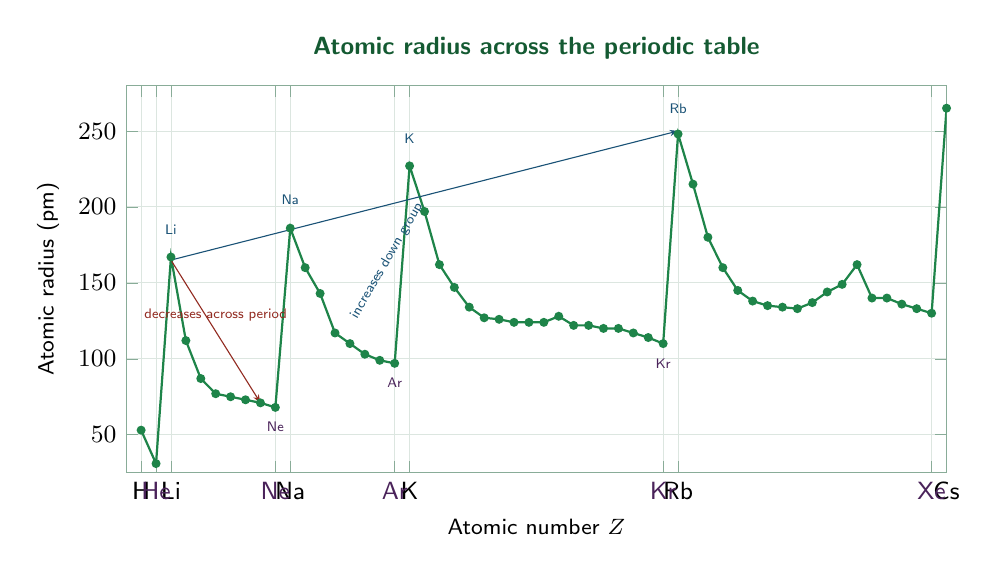
\begin{tikzpicture}[every node/.style={font=\sffamily\small}]
  \begin{axis}[
    width=12cm, height=6.5cm,
    xlabel={Atomic number $Z$},
    ylabel={Atomic radius (pm)},
    xmin=0, xmax=55,
    ymin=25, ymax=280,
    xtick={1,3,11,19,37,55},
    xticklabels={H,Li,Na,K,Rb,Cs},
    extra x ticks={2,10,18,36,54},
    extra x tick labels={He,Ne,Ar,Kr,Xe},
    extra x tick style={tick label style={color=ProblemColor}},
    ytick={50,100,150,200,250},
    grid=both,
    grid style={line width=0.3pt, draw=JourneyColor!15},
    axis line style={color=JourneyColor!50},
    tick style={color=JourneyColor!50},
    title style={font=\sffamily\small\bfseries, color=JourneyColor},
    title={Atomic radius across the periodic table},
    label style={font=\sffamily\footnotesize}
  ]
    \addplot[thick, color=ModuleColor, mark=*, mark size=1.2pt]
      coordinates {
        (1,53)(2,31)(3,167)(4,112)(5,87)(6,77)(7,75)(8,73)(9,71)
        (10,68)(11,186)(12,160)(13,143)(14,117)(15,110)(16,103)(17,99)
        (18,97)(19,227)(20,197)(21,162)(22,147)(23,134)(24,127)(25,126)
        (26,124)(27,124)(28,124)(29,128)(30,122)(31,122)(32,120)(33,120)
        (34,117)(35,114)(36,110)(37,248)(38,215)(39,180)(40,160)(41,145)
        (42,138)(43,135)(44,134)(45,133)(46,137)(47,144)(48,149)(49,162)
        (50,140)(51,140)(52,136)(53,133)(54,130)(55,265)
      };

    % Annotations: peaks = alkali metals
    \node[font=\sffamily\tiny, text=TrendDown]
      at (axis cs:3,185) {Li};
    \node[font=\sffamily\tiny, text=TrendDown]
      at (axis cs:11,205) {Na};
    \node[font=\sffamily\tiny, text=TrendDown]
      at (axis cs:19,245) {K};
    \node[font=\sffamily\tiny, text=TrendDown]
      at (axis cs:37,265) {Rb};

    % Annotation: troughs = noble gases (smallest in period)
    \node[font=\sffamily\tiny, text=ProblemColor]
      at (axis cs:10,55) {Ne};
    \node[font=\sffamily\tiny, text=ProblemColor]
      at (axis cs:18,84) {Ar};
    \node[font=\sffamily\tiny, text=ProblemColor]
      at (axis cs:36,97) {Kr};

    % Trend arrows
    \draw[-{Stealth[length=3pt]}, thin, TrendUp]
      (axis cs:3,165) -- (axis cs:9,71)
      node[midway, above, font=\sffamily\tiny, text=TrendUp]
        {decreases across period};
    \draw[-{Stealth[length=3pt]}, thin, TrendDown]
      (axis cs:3,165) -- (axis cs:37,250)
      node[midway, left, font=\sffamily\tiny, text=TrendDown, rotate=60]
        {increases down group};
  \end{axis}
\end{tikzpicture}
\end{center}

\vspace{0.4em}

The sawtooth pattern is striking:
\begin{itemize}[nosep, leftmargin=2em]
  \item \textbf{Across a period:} radius \emph{decreases}.
        $Z_\text{eff}$ increases (poor same-shell shielding),
        pulling electrons inward.
  \item \textbf{Down a group:} radius \emph{increases}.
        A new shell is added, placing electrons farther out.
  \item \textbf{Peaks:} alkali metals (new shell starts,
        single electron far from nucleus).
  \item \textbf{Troughs within periods:} noble gases
        (highest $Z_\text{eff}$ in period, electrons
        pulled tightest).
\end{itemize}

% ─── Section: Ionisation Energy ──────────────────────────────────────────────
\subsection{Ionisation Energy}

The \newterm{first ionisation energy} (IE$_1$) is the
energy to remove the least-tightly-held electron:
\[
  \text{X}(g) \to \text{X}^+(g) + e^- \qquad \Delta E = \text{IE}_1
\]

IE follows the same logic as radius but in reverse:
\begin{itemize}[nosep, leftmargin=2em]
  \item \textbf{Across a period:} IE generally \emph{increases}
        (higher $Z_\text{eff}$ holds electrons more tightly).
  \item \textbf{Down a group:} IE \emph{decreases}
        (outer electrons farther away, more shielded).
\end{itemize}

But there are two important anomalies within periods:

\subsubsection{Anomaly 1: Group 2 to Group 13 (e.g.\ Be to B)}

Boron (B, $2s^22p^1$) has \emph{lower} IE than
beryllium (Be, $2s^2$), even though B has higher $Z$.

Reason: B's outermost electron is in a $2p$ orbital,
which is higher in energy (less penetrating, more shielded)
than Be's $2s$ electrons.
Removing a $2p$ electron is easier than removing a $2s$ electron.

\subsubsection{Anomaly 2: Group 15 to Group 16 (e.g.\ N to O)}

Oxygen (O, $2s^22p^4$) has \emph{lower} IE than
nitrogen (N, $2s^22p^3$), even though O has higher $Z$.

Reason: O's fourth $2p$ electron must share an orbital
with another electron (Pauli).
Electron-electron repulsion in the paired orbital
destabilises it, making it easier to remove.
N's half-filled $2p^3$ (one electron per orbital) is
extra-stable (Hund's rule).

\begin{center}
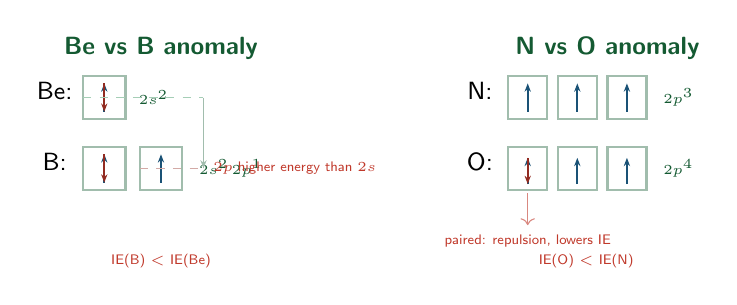
\begin{tikzpicture}[every node/.style={font=\sffamily\small}, scale=0.9]

  % Be vs B anomaly
  \begin{scope}[xshift=-4.0cm]
    \node[font=\sffamily\small\bfseries, color=JourneyColor]
      at (1.2, 2.8) {Be vs B anomaly};
    % Be: 2s2
    \node at (-0.3, 2.2) {Be:};
    \draw[thick, JourneyColor!40] (0.1,1.8) rectangle (0.7,2.4);
    \draw[-{Stealth[length=3pt]}, thick, TrendDown] (0.4,1.9) -- (0.4,2.3);
    \draw[-{Stealth[length=3pt]}, thick, TrendUp]   (0.4,2.3) -- (0.4,1.9);
    \node[right, font=\sffamily\tiny, color=JourneyColor] at (0.75,2.1) {$2s^2$};
    % B: 2s2 2p1
    \node at (-0.3, 1.2) {B:};
    \draw[thick, JourneyColor!40] (0.1,0.8) rectangle (0.7,1.4);
    \draw[-{Stealth[length=3pt]}, thick, TrendDown] (0.4,0.9) -- (0.4,1.3);
    \draw[-{Stealth[length=3pt]}, thick, TrendUp]   (0.4,1.3) -- (0.4,0.9);
    \draw[thick, JourneyColor!40] (0.9,0.8) rectangle (1.5,1.4);
    \draw[-{Stealth[length=3pt]}, thick, TrendDown] (1.2,0.9) -- (1.2,1.3);
    \node[right, font=\sffamily\tiny, color=JourneyColor] at (1.6,1.1) {$2s^2\,2p^1$};
    % Energy level lines
    \draw[thin, ModuleColor!40, dashed] (0.1,2.1) -- (1.8,2.1);
    \draw[thin, TrendUp!40, dashed]     (0.9,1.1) -- (1.8,1.1);
    % Arrow
    \draw[-{Stealth[length=3pt]}, thin, JourneyColor!40]
      (1.8,2.1) -- (1.8,1.1)
      node[right, font=\sffamily\tiny, text=WarningColor]
        {$2p$ higher energy than $2s$};
    \node[font=\sffamily\tiny, text=WarningColor]
      at (1.2,-0.2) {IE(B) $<$ IE(Be)};
  \end{scope}

  % N vs O anomaly
  \begin{scope}[xshift=2.0cm]
    \node[font=\sffamily\small\bfseries, color=JourneyColor]
      at (1.5, 2.8) {N vs O anomaly};
    % N: 2p3 (one per orbital)
    \node at (-0.3, 2.2) {N:};
    \foreach \x in {0.1, 0.8, 1.5} {
      \draw[thick, JourneyColor!40] (\x,1.8) rectangle (\x+0.55,2.4);
      \draw[-{Stealth[length=3pt]}, thick, TrendDown]
        (\x+0.275,1.9) -- (\x+0.275,2.3);
    }
    \node[right, font=\sffamily\tiny, color=JourneyColor] at (2.15,2.1) {$2p^3$};
    % O: 2p4 (one paired)
    \node at (-0.3, 1.2) {O:};
    \draw[thick, JourneyColor!40] (0.1,0.8) rectangle (0.65,1.4);
    \draw[-{Stealth[length=3pt]}, thick, TrendDown] (0.375,0.88) -- (0.375,1.25);
    \draw[-{Stealth[length=3pt]}, thick, TrendUp]   (0.375,1.25) -- (0.375,0.88);
    \foreach \x in {0.8, 1.5} {
      \draw[thick, JourneyColor!40] (\x,0.8) rectangle (\x+0.55,1.4);
      \draw[-{Stealth[length=3pt]}, thick, TrendDown]
        (\x+0.275,0.88) -- (\x+0.275,1.25);
    }
    \node[right, font=\sffamily\tiny, color=JourneyColor] at (2.15,1.1) {$2p^4$};
    % Annotation
    \draw[thin, WarningColor!60, ->]
      (0.375, 0.75) -- (0.375, 0.3)
      node[below, font=\sffamily\tiny, text=WarningColor]
        {paired: repulsion, lowers IE};
    \node[font=\sffamily\tiny, text=WarningColor]
      at (1.2,-0.2) {IE(O) $<$ IE(N)};
  \end{scope}

\end{tikzpicture}
\end{center}

% ─── Section: Electron Affinity ──────────────────────────────────────────────
\subsection{Electron Affinity}

The \newterm{electron affinity} (EA) is the energy
released when a neutral atom gains an electron:
\[
  \text{X}(g) + e^- \to \text{X}^-(g) \qquad \Delta E = -\text{EA}
\]

A large positive EA means the atom strongly attracts electrons.
The trend: EA generally increases across a period and
decreases down a group --- similar to IE.

Notable values:
\begin{center}
\small
\begin{tabular}{lccccccc}
\toprule
Element & F & Cl & O & S & N & Ne & Na \\
\midrule
EA (eV) & 3.45 & 3.61 & 1.46 & 2.08 & $-0.07$ & $-0.22$ & 0.55 \\
\bottomrule
\end{tabular}
\end{center}

Chlorine has a higher EA than fluorine because F is so
small that the added electron experiences strong
repulsion from existing electrons.
Nitrogen has a \emph{negative} EA (it repels an extra electron)
because its half-filled $2p^3$ is extra-stable.

% ─── Section: Electronegativity ──────────────────────────────────────────────
\subsection{Electronegativity: Combining IE and EA}

\newterm{Electronegativity} ($\chi$) is a measure of
an atom's ability to attract electrons within a bond.
It is not directly measurable, but several scales exist.

The most widely used is the \newterm{Pauling scale}
(based on bond energies) and the Mulliken approximation:
\[
  \chi_\text{Mulliken} \approx \frac{\text{IE} + \text{EA}}{2}
\]

\begin{center}
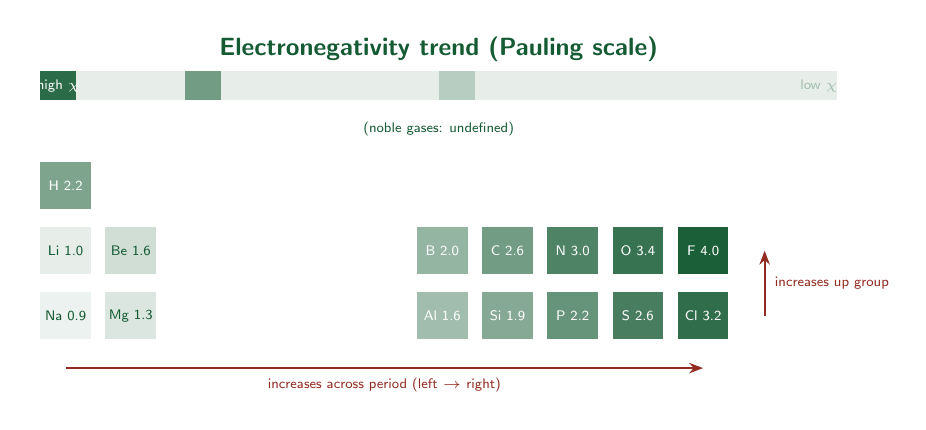
\begin{tikzpicture}[every node/.style={font=\sffamily\small},
                    scale=0.92]

  % Simplified periodic table showing electronegativity as shading
  % Period 2 and 3 elements, Groups 1-18
  \node[font=\sffamily\small\bfseries, color=JourneyColor]
    at (5.5, 4.0) {Electronegativity trend (Pauling scale)};

  % Color gradient description
  \fill[JourneyColor!10] (0.0,3.3) rectangle (11.0,3.7);
  \fill[JourneyColor!90] (0.0,3.3) rectangle (0.5,3.7);
  \fill[JourneyColor!60] (2.0,3.3) rectangle (2.5,3.7);
  \fill[JourneyColor!30] (5.5,3.3) rectangle (6.0,3.7);
  \fill[JourneyColor!10] (10.5,3.3) rectangle (11.0,3.7);
  \node[font=\sffamily\tiny, text=white] at (0.25, 3.5) {high $\chi$};
  \node[font=\sffamily\tiny, text=JourneyColor!40] at (10.75, 3.5) {low $\chi$};
  \node[font=\sffamily\tiny, text=JourneyColor] at (5.5, 2.9) {(noble gases: undefined)};

  % Row 1
  \pgfmathsetmacro{\yR}{1.8}
  % H (chi=2.2) - mid-dark
  \fill[JourneyColor!55] (0.0,\yR) rectangle (0.7,\yR+0.65);
  \node[font=\sffamily\tiny, text=white] at (0.35,\yR+0.32) {H 2.2};
  % Li (0.98)
  \fill[JourneyColor!10] (0.0,0.9) rectangle (0.7,1.55);
  \node[font=\sffamily\tiny, text=JourneyColor] at (0.35,1.22) {Li 1.0};
  % Be (1.57)
  \fill[JourneyColor!20] (0.9,0.9) rectangle (1.6,1.55);
  \node[font=\sffamily\tiny, text=JourneyColor] at (1.25,1.22) {Be 1.6};
  % B (2.04)
  \fill[JourneyColor!45] (5.2,0.9) rectangle (5.9,1.55);
  \node[font=\sffamily\tiny, text=white] at (5.55,1.22) {B 2.0};
  % C (2.55)
  \fill[JourneyColor!60] (6.1,0.9) rectangle (6.8,1.55);
  \node[font=\sffamily\tiny, text=white] at (6.45,1.22) {C 2.6};
  % N (3.04)
  \fill[JourneyColor!75] (7.0,0.9) rectangle (7.7,1.55);
  \node[font=\sffamily\tiny, text=white] at (7.35,1.22) {N 3.0};
  % O (3.44)
  \fill[JourneyColor!85] (7.9,0.9) rectangle (8.6,1.55);
  \node[font=\sffamily\tiny, text=white] at (8.25,1.22) {O 3.4};
  % F (3.98) - darkest
  \fill[JourneyColor!97] (8.8,0.9) rectangle (9.5,1.55);
  \node[font=\sffamily\tiny, text=white] at (9.15,1.22) {F 4.0};

  % Row 3 (Na-Cl)
  \fill[JourneyColor!8]  (0.0,0.0) rectangle (0.7,0.65);
  \node[font=\sffamily\tiny, text=JourneyColor] at (0.35,0.32) {Na 0.9};
  \fill[JourneyColor!15] (0.9,0.0) rectangle (1.6,0.65);
  \node[font=\sffamily\tiny, text=JourneyColor] at (1.25,0.32) {Mg 1.3};
  \fill[JourneyColor!40] (5.2,0.0) rectangle (5.9,0.65);
  \node[font=\sffamily\tiny, text=white] at (5.55,0.32) {Al 1.6};
  \fill[JourneyColor!52] (6.1,0.0) rectangle (6.8,0.65);
  \node[font=\sffamily\tiny, text=white] at (6.45,0.32) {Si 1.9};
  \fill[JourneyColor!65] (7.0,0.0) rectangle (7.7,0.65);
  \node[font=\sffamily\tiny, text=white] at (7.35,0.32) {P 2.2};
  \fill[JourneyColor!78] (7.9,0.0) rectangle (8.6,0.65);
  \node[font=\sffamily\tiny, text=white] at (8.25,0.32) {S 2.6};
  \fill[JourneyColor!88] (8.8,0.0) rectangle (9.5,0.65);
  \node[font=\sffamily\tiny, text=white] at (9.15,0.32) {Cl 3.2};

  % Trend arrows
  \draw[-{Stealth[length=5pt]}, thick, TrendUp]
    (10.0,0.32) -- (10.0,1.22)
    node[midway, right, font=\sffamily\tiny, text=TrendUp]
      {increases up group};
  \draw[-{Stealth[length=5pt]}, thick, TrendUp]
    (0.35,-0.4) -- (9.15,-0.4)
    node[midway, below, font=\sffamily\tiny, text=TrendUp]
      {increases across period (left $\to$ right)};

\end{tikzpicture}
\end{center}

\vspace{0.4em}

Fluorine ($\chi = 3.98$) is the most electronegative element.
Francium ($\chi \approx 0.7$) is the least electronegative metal.
The difference in electronegativity between bonded atoms
determines the bond character:
$\Delta\chi < 0.5$: covalent; $0.5 < \Delta\chi < 1.7$: polar covalent;
$\Delta\chi > 1.7$: ionic.

% ─── Section: Summary of Trends ─────────────────────────────────────────────
\subsection{Summary: The Trend Map}

\begin{center}
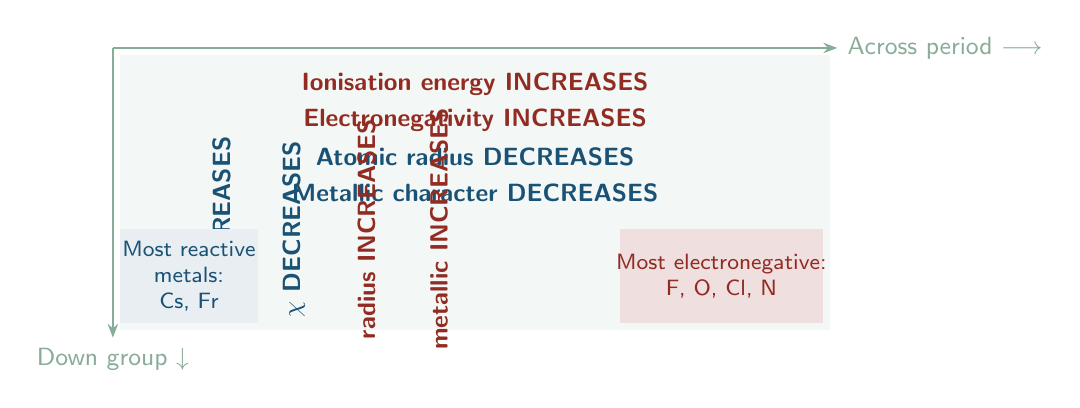
\begin{tikzpicture}[every node/.style={font=\sffamily\small, align=center},
                    scale=0.92]

  % Axes of the table
  \draw[-{Stealth[length=5pt]}, thick, JourneyColor!50]
    (0,0) -- (10,0) node[right] {Across period $\longrightarrow$};
  \draw[-{Stealth[length=5pt]}, thick, JourneyColor!50]
    (0,0) -- (0,-4) node[below] {Down group $\downarrow$};

  % Grid of cells (simplified)
  \fill[JourneyColor!5] (0.1,-0.1) rectangle (9.9,-3.9);

  % Trend labels
  \node[font=\sffamily\small\bfseries, text=TrendUp]
    at (5.0,-0.5) {Ionisation energy INCREASES};
  \node[font=\sffamily\small\bfseries, text=TrendUp]
    at (5.0,-1.0) {Electronegativity INCREASES};
  \node[font=\sffamily\small\bfseries, text=TrendDown]
    at (5.0,-1.5) {Atomic radius DECREASES};
  \node[font=\sffamily\small\bfseries, text=TrendDown]
    at (5.0,-2.0) {Metallic character DECREASES};

  \node[font=\sffamily\small\bfseries, text=TrendDown, rotate=90]
    at (1.5,-2.5) {IE DECREASES};
  \node[font=\sffamily\small\bfseries, text=TrendDown, rotate=90]
    at (2.5,-2.5) {$\chi$ DECREASES};
  \node[font=\sffamily\small\bfseries, text=TrendUp, rotate=90]
    at (3.5,-2.5) {radius INCREASES};
  \node[font=\sffamily\small\bfseries, text=TrendUp, rotate=90]
    at (4.5,-2.5) {metallic INCREASES};

  % Corner annotations
  \fill[TrendUp!15] (7.0,-2.5) rectangle (9.8,-3.8);
  \node[font=\sffamily\footnotesize, text=TrendUp]
    at (8.4,-3.15) {Most electronegative:\\F, O, Cl, N};

  \fill[TrendDown!10] (0.1,-2.5) rectangle (2.0,-3.8);
  \node[font=\sffamily\footnotesize, text=TrendDown]
    at (1.05,-3.15) {Most reactive\\metals:\\Cs, Fr};

\end{tikzpicture}
\end{center}

\begin{problembox}
\begin{enumerate}[label=\textbf{\arabic*.}]
  \item Arrange each set in order of increasing first
        ionisation energy, then explain using $Z_\text{eff}$:
        \begin{enumerate}[label=(\alph*)]
          \item Na, Mg, Al, Si, P, S, Cl, Ar
          \item Li, Na, K, Rb, Cs
          \item O, S, Se, Te
        \end{enumerate}

  \item The first five ionisation energies of an unknown
        element X are:
        \begin{center}
        786, 1577, 3232, 4356, 16\,000 kJ/mol
        \end{center}
        \begin{enumerate}[label=(\alph*)]
          \item Identify the group of element X.
                Explain your reasoning from the data.
          \item Identify two possible elements that could be X.
          \item Sketch the electron configuration of X.
        \end{enumerate}

  \item Slater's rules give the shielding constant as:
        For an electron in the $n$th shell:
        electrons in the same shell contribute 0.35 each;
        electrons in the $(n-1)$th shell contribute 0.85 each;
        electrons in lower shells contribute 1.00 each.
        \begin{enumerate}[label=(\alph*)]
          \item Calculate $Z_\text{eff}$ for the outermost
                electron in: Na, Cl, K, Fe (use the 4s electron).
          \item The atomic radii of Na and Cl are 186 pm
                and 99 pm respectively.
                For hydrogen-like orbitals, $r \propto n^2/Z_\text{eff}$.
                Using this, predict the ratio of the
                covalent radii of Na to Cl from their $Z_\text{eff}$.
                Compare to the actual ratio.
        \end{enumerate}
\end{enumerate}
\end{problembox}

% ─── Section: Oxidation States and Valence ────────────────────────────────────
\subsection{Oxidation States and Valence: The Chemistry of Position}

The periodic table position predicts not just atomic properties
but the chemistry the element will do.

The \newterm{valence} --- the number of bonds an atom forms ---
is directly related to the number of unpaired valence electrons
or the number of electrons needed to complete a shell.

\begin{center}
\small
\begin{tabular}{lllll}
\toprule
Group & Valence electrons & Common valence & Formula type & Example \\
\midrule
1  & $ns^1$       & 1 & MX, M$_2$O & \ce{NaCl}, \ce{Na2O} \\
2  & $ns^2$       & 2 & MX$_2$, MO & \ce{MgCl2}, \ce{MgO} \\
13 & $ns^2np^1$   & 3 & MX$_3$, M$_2$O$_3$ & \ce{AlCl3}, \ce{Al2O3} \\
14 & $ns^2np^2$   & 4 & MX$_4$, MO$_2$ & \ce{CCl4}, \ce{SiO2} \\
15 & $ns^2np^3$   & 3 & MH$_3$, M$_2$O$_3$ & \ce{NH3}, \ce{P4O6} \\
16 & $ns^2np^4$   & 2 & MH$_2$, MO$_2$ & \ce{H2O}, \ce{SO2} \\
17 & $ns^2np^5$   & 1 & MH, MX & \ce{HCl}, \ce{NaCl} \\
18 & $ns^2np^6$   & 0 & --- & \ce{Ne}, \ce{Ar} \\
\bottomrule
\end{tabular}
\end{center}

\vspace{0.5em}

The pattern for Groups 1--2 and 13--18 is straightforward.
Notice that Groups 15--17 can also exhibit higher oxidation
states when the central atom is large enough
(e.g.\ \ce{PCl5}, oxidation state +5; \ce{SF6}, +6)
by using $d$ orbitals.

% ─── Section: Deep Problems ──────────────────────────────────────────────────
\subsection*{Deep Problems}

\begin{deepbox}
\begin{enumerate}[label=\textbf{D\arabic*.}]

  \item \textbf{Relativistic Effects and the Colour of Gold.}

        For heavy elements ($Z > 70$), electrons in inner
        $s$ orbitals move at speeds approaching $c$.
        Relativistic mass increase causes these orbitals
        to contract.
        For gold ($Z=79$), the $6s$ orbital is $\sim$20\%
        smaller than its non-relativistic value.

        \begin{enumerate}[label=(\alph*)]
          \item The non-relativistic energy of the gold
                $6s$ orbital would be around $-5.5$ eV.
                Relativistic contraction raises the effective
                nuclear charge seen by the $6s$ electrons.
                Explain qualitatively why contraction of inner
                $s$ orbitals causes the valence $6s$ to
                also contract and lower in energy.
          \item The $5d$ orbitals of gold are indirectly
                expanded by the $6s$ contraction
                (better shielding from the $6s$).
                The $5d$--$6s$ energy gap in gold is
                $\sim 2.4$ eV, corresponding to light
                of wavelength $\sim 517$ nm (blue-green).
          \item Gold absorbs blue-green light and reflects
                red and yellow light.
                Silver and platinum have larger $5d$--$6s$
                gaps (absorbed in the UV), so they appear
                grey-white.
                Explain why gold is gold-coloured and silver
                is not, using this energy gap argument.
          \item Mercury is liquid at room temperature
                (m.p.\ $-39$\textdegree C) while all other
                transition metals are solid.
                Using the same relativistic argument,
                explain why Hg-Hg bonds are very weak
                (Hg: $[Xe]\,4f^{14}\,5d^{10}\,6s^2$,
                fully filled, small $6s$ orbital).
        \end{enumerate}

  \item \textbf{Ionisation Energy and Electronegativity from First Principles.}

        For a hydrogen-like atom with nuclear charge $Z_\text{eff}$,
        the energy of the outermost electron in shell $n$ is:
        \[
          E_n = -\frac{13.6\,Z_\text{eff}^2}{n^2}\ \text{eV}
        \]

        \begin{enumerate}[label=(\alph*)]
          \item Using Slater's rules from Problem 3, calculate
                $Z_\text{eff}$ for the outermost electron in
                each of the Period 3 elements (Na through Ar).
          \item Calculate the predicted IE for each.
          \item Compare to measured values:
                Na~5.1, Mg~7.6, Al~6.0, Si~8.2,
                P~10.5, S~10.4, Cl~13.0, Ar~15.8 (all in eV).
          \item Where does the prediction work well?
                Where does it fail?
                The large failure at Al and S corresponds
                to the two IE anomalies.
                Do the anomalies still appear in the predicted
                values, or does the model miss them?
          \item What missing physics causes the discrepancies?
        \end{enumerate}

\end{enumerate}
\end{deepbox}

% ─── Reflection ──────────────────────────────────────────────────────────────
\subsection*{Reflection}

\begin{reflectionbox}
\begin{enumerate}[label=\textbf{R\arabic*.}]
  \item All periodic trends ultimately reduce to
        $Z_\text{eff}$ and orbital radius.
        \textbf{Is this satisfying, or does it feel like
        we've just pushed the complexity one level deeper?}
        What would it mean to fully ``explain'' a periodic trend?

  \item The anomalies (Be/B and N/O ionisation energies)
        are actually very useful pedagogically ---
        they prevent the trend from being merely a
        memorisation exercise.
        \textbf{What role do exceptions play in science?}
        Are they failures of the theory,
        or evidence that the theory is deep enough to have
        non-trivial consequences?

  \item Gold's colour is a relativistic effect.
        \textbf{What does it mean that a macroscopic, observable
        property of matter (its colour, visible to the naked eye)
        requires special relativity to explain?}
        How many other everyday phenomena have similarly
        deep physical origins that we usually take for granted?
\end{enumerate}
\end{reflectionbox}

\vspace{1.5em}
\begin{center}
\begin{tcolorbox}[enhanced, colback=DiscoveryColor!8, colframe=DiscoveryColor,
  width=0.88\textwidth, arc=3pt]
\centering\sffamily\small
\textbf{What we invented in this module.}\\[4pt]
We invented $Z_\text{eff}$ --- the single concept that unifies
all periodic trends.
Atomic radius, ionisation energy, electron affinity, and
electronegativity are all different faces of the same
underlying physics: how strongly the nucleus holds its
outermost electrons, after shielding by inner shells.
The two anomalies (B/Be and O/N) are not failures of the theory
but confirmations of it: they arise from the $s/p$ energy
splitting and Hund's rule, both of which we derived in Journey~2.
The periodic table is not memorisation.
It is a consequence of quantum mechanics.
\end{tcolorbox}
\end{center}

\vspace{2em}
\noindent\textcolor{JourneyColor!40}{\rule{\textwidth}{0.6pt}}
\begin{center}
\textit{\sffamily\small
Module 3.2 complete. Continue to Module 3.3:\\
\textbf{The Noble Gases: A Group Nobody Predicted}.}
\end{center}

\end{document}